\documentclass[12pt]{article}
\usepackage[english]{babel}
\usepackage[utf8]{inputenc}
\usepackage{graphicx}
\usepackage{float}
\usepackage[margin=1in]{geometry}
\title{CR1}
\author{Benoit Viguier}
\date{11/10/2014}
\begin{document}
\section{State of Art on MCTS}
\subsection{History of computers vs Humans}
In 1997, Deep Blue a computer built by IBM won a six games match against the current chess world champion Garry Kasparov. Humans got beaten on Chess, but remain undefeated on Go, therefore the research has switched to that game. Until 2002, methods based on decompositions and positions evaluations were used in order to solve such games. From 2002 to 2005 the Monte Carlo algorithm was used in order to find the best moves. Since 2006, it's implementation in a tree (MCTS) has been developped, rocketing the results in term of Artificial Intelligence on Go. On june 5th, 2013, Zen a Go programm defeated Takuto Ooomote (9 Dan) with a 3 stone handicap.
\begin{figure}[H]
\centering
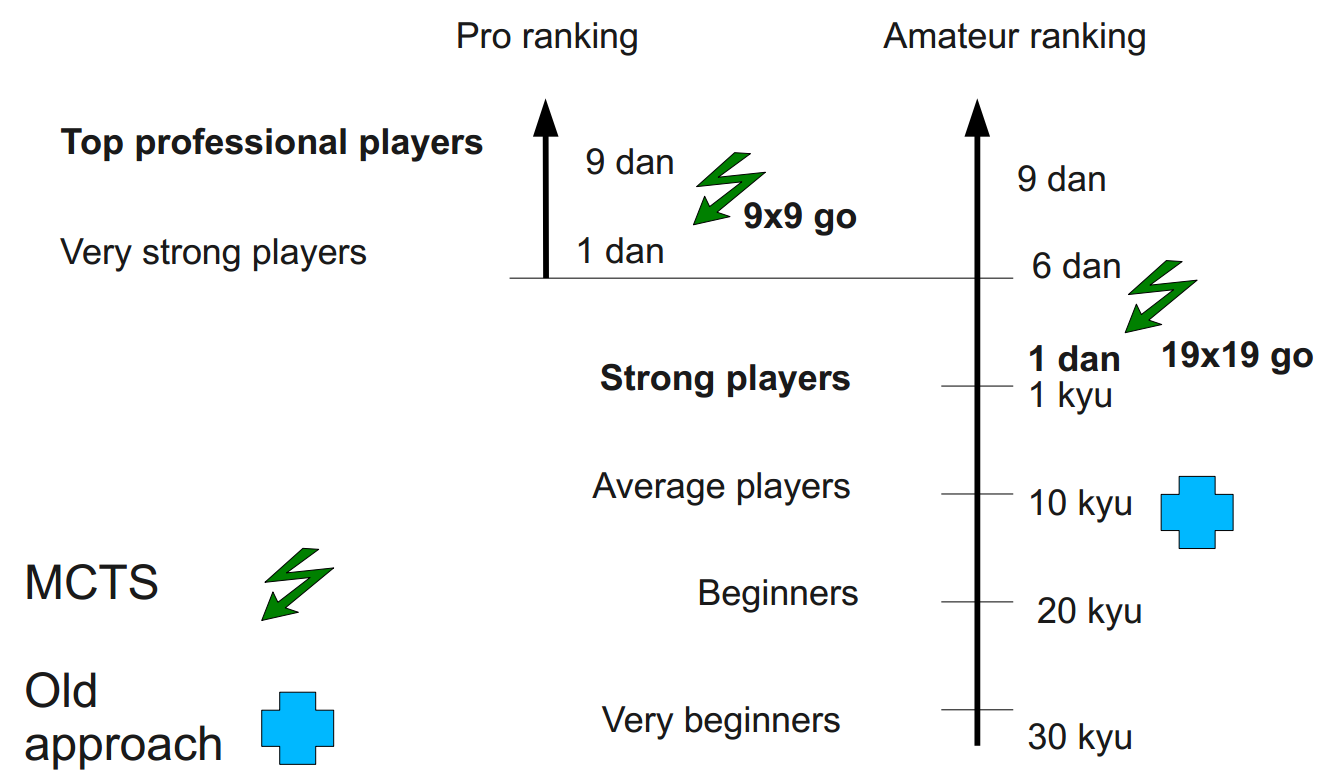
\includegraphics[width=12cm]{img/ranking.png}
\caption{\label{fig:ranking}Comparison between Go algorithms and human skill (\textit{2011}).}
\end{figure}
\textit{The ranking system of the game of Go is the following : kyu are for students ranks, Dan are masters ranks. Beginners start at 30 kyu and advance downward the kyu grades. Once one ranks over 1 kyu, he will receive the 1st Dan (as the black belt in Judo) and will move upward through the Dan ranks until the 9th.}\\
However MCTS wasn't the first method applied in order to solve Arimaa, the \ensuremath{\alpha\beta} method was used first. At the moment the top programms (Bomb by David Fotland : 2002 to 2008, Clueless by Jeff Bacher 2009) are ranked about 1800 elo. For comparison, strongest humans players are rated around 2450 elo. (source : Method of MCTS and the Game Arimaa, Tomas Kozelek, 2009, Master's Thesis).
\medskip

\textit{The Elo rating system is a method for calculating the relative skill levels of players in competitor-versus-competitor games such as chess. It use also used for Arimaa. Beginers rank around 1200 elo, experts around 200 elo and International Masters over 2400 elo.}
\newpage
\subsection{The minimax algorithm}
The minimax algorithm is a way of finding an optimal move in a two player game. In the search tree for a two-player game, there are two kinds of nodes, nodes representing \textit{your} moves and nodes representing your \textit{opponent}'s moves.
\begin{figure}[H]
\centering
	\begin{minipage}[b]{0.45\linewidth}
		\centering
		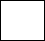
\includegraphics[height=1cm]{img/max.png}
		\caption{\label{fig:max}Nodes representing your moves are generally drawn as squares, these are also called MAX nodes.}
	\end{minipage}%
	\hspace*{1cm}
	\begin{minipage}[b]{0.45\linewidth}
		\centering
		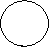
\includegraphics[height=1cm]{img/min.png}
		\caption{\label{fig:min}Nodes representing your opponent's moves are generally drawn as circles, these are also called MIN nodes.}
	\end{minipage}%
\end{figure}
\noindent
The goal at a MAX/MIN node is to maximize/minimize the value of the subtree rooted at that node. To do this, a MAX/MIN node chooses the child with the greatest/smallest value, and that becomes the value of the MAX/MIN node.\\
Note that it's typical for two player games to have different branching factors at each node. The move I make could make restrictions on what moves are possible for the other player, or possibly remove restrictions. Note also that in this example, we're ignoring what the game or the probem space are in order to focus on the algorithm.

\begin{figure}[H]
\centering
	\begin{minipage}[b]{0.45\linewidth}
		\centering
		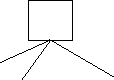
\includegraphics[height=1.5cm]{img/minimax2.png}
		\caption{\label{fig:minimax2}When we start the problem, all minimax sees is the start node.}
	\end{minipage}%
	\hspace*{1cm}
	\begin{minipage}[b]{0.45\linewidth}
		\centering
		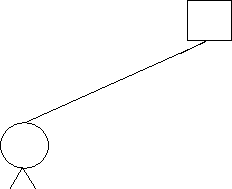
\includegraphics[height=3cm]{img/minimax3.png}
		\caption{\label{fig:minimax3}It begins like a depth first search, generating the first child.}
	\end{minipage}%
\end{figure}

\noindent
So far we've really seen no evaluation values. The way minimax works is to go down a specified number of full moves (where one ``full move'' is actually a move by you and a move by your opponent), then calculate evaluation values for states at that depth. For this example, we're going to go down one full move, which is one more level. 
\begin{figure}[H]
\centering
	\begin{minipage}[b]{0.45\linewidth}
		\centering
		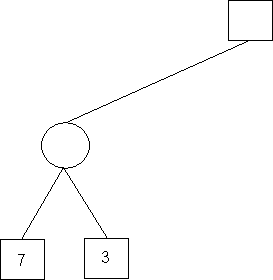
\includegraphics[height=3cm]{img/minimax4.png}
		\caption{\label{fig:minimax4}we generate the values for those nodes.}
	\end{minipage}%
	\hspace*{1cm}
	\begin{minipage}[b]{0.45\linewidth}
		\centering
		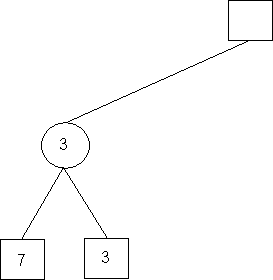
\includegraphics[height=3cm]{img/minimax5.png}
		\caption{\label{fig:minimax5}It chooses the minimum of the two child node values, which is 3.}
	\end{minipage}%
\end{figure}

\noindent
The max node at the top still has two other children nodes that we need to generate and search.

\begin{figure}[H]
\centering
	\begin{minipage}[b]{0.45\linewidth}
		\centering
		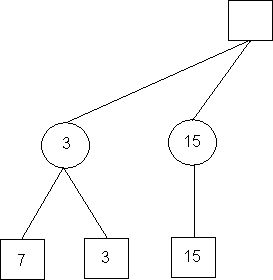
\includegraphics[height=3cm]{img/minimax6.png}
		\caption{\label{fig:minimax6}Since there is only one child, the min node must take it's value.}
		\end{minipage}%
	\hspace*{1cm}
	\begin{minipage}[b]{0.45\linewidth}
		\centering
		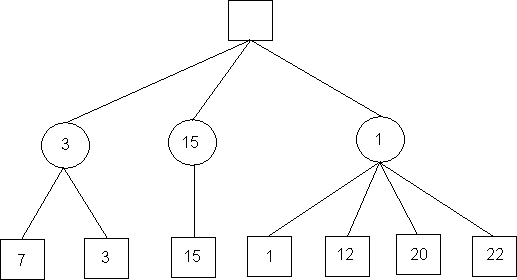
\includegraphics[height=3cm]{img/minimax8.png}
		\caption{\label{fig:minimax8}The third min node chooses the minimum of it's child node values, 1.}
	\end{minipage}%
\end{figure}

\noindent
Finally we have all of the values of the children of the max node at the top level, so it chooses the maximum of them, 15, and we get the final solution. 

\begin{figure}[H]
\centering
	\begin{minipage}[b]{1\linewidth}
		\centering
		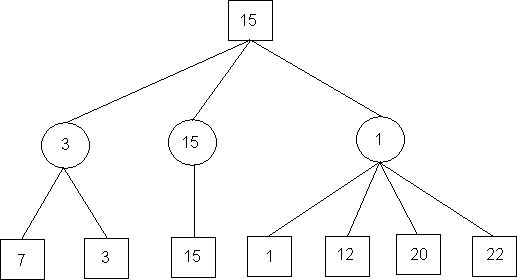
\includegraphics[height=3cm]{img/minimax9.png}
		\caption{\label{fig:minimax9}Final tree.}
	\end{minipage}%
\end{figure}

\noindent
What this tells us is that we should take the move that leads to the middle min node, since it'll lead to the best possible state for us one full move down the road. 

\subsection{The \ensuremath{\alpha\beta} pruning} %pruning = elaguage en anglais
The \ensuremath{\alpha\beta} method is a search algorithm that decrease the number of leaf that will be explored by the minimax algorithm. That way, the size of the tree will be smaller, the algorithm will be able to dive further and the time spend on more interesting subtree is greater.\\
If the leaf's position is less interesting than its parents, the algorithm won't explore anyfurther.

\end{document}